\documentclass{scrartcl}

\usepackage{array}
\usepackage{bytefield}
\usepackage{fontspec}
\usepackage{gitinfo2}
\usepackage{graphicx}
\usepackage{hyperref}
\usepackage{listings}
\usepackage{microtype}
\usepackage{polyglossia}
\usepackage{scrlayer-scrpage}
\usepackage{xcolor}

\linespread{1.3}

\setmainlanguage{lithuanian}

\addtokomafont{disposition}{\rmfamily}

\setmainfont{TeX Gyre Termes}
\setmonofont{TeX Gyre Cursor}

\ohead{Release \gitDescribe\ (\gitCommitterDate)}
\cfoot*{\pagemark}

\newcolumntype{?}{!{\vrule width 1pt}}

\definecolor{lightgray}{gray}{0.8}

\setlength{\headheight}{\baselineskip}
\setlength{\footheight}{\baselineskip}

\lstset{
    basicstyle = \footnotesize\ttfamily,%
    escapeinside = {/*}{*/},%
    firstnumber = 1,%
    numbers = left%
}

\graphicspath{{images/}}

\begin{document}
    \newcommand{\instr}[3]{\subparagraph{\makebox[6em][l]{\texttt{#1}}} (\texttt{#2})\par#3\par}
    \begin{titlepage}
        \begin{center}
            VILNIAUS UNIVERSITETAS \\
            MATEMATIKOS IR INFORMATIKOS FAKULTETAS \\
            \vspace{4cm}
            \Large\textbf{Virtualios ir realios mašinos projektas}
        \end{center}
        \vspace{4cm}
        \begin{flushright}
            \begin{tabular}[t]{l}
                Atliko: 3 kurso studentai \\
                Tautvydas Baliukynas \\
                Edvinas Gervelis \\
                Ernestas Kulik \\
                Justinas Valatkevičius
            \end{tabular}
        \end{flushright}
        \vspace*{\fill}
        \begin{center}
            \large{Vilnius \\ 2018}
        \end{center}
    \end{titlepage}
    \section{Reali mašina}
        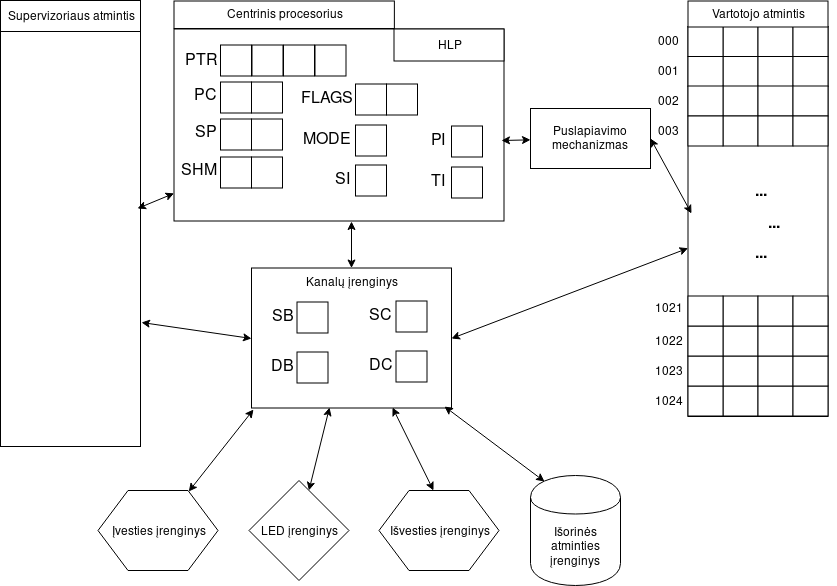
\includegraphics[width=\textwidth]{RM_model}
        \subsection{Procesorius}
            \subsubsection{Registrai}
                \paragraph{\makebox[3em][l]{PC}} Programų skaitiklis.
                \paragraph{\makebox[3em][l]{SP}} Steko nuoroda.
                \paragraph{\makebox[3em][l]{FLAGS}} Paskutinės aritmetinės ar loginės operacijos požymiai.
                \paragraph{\makebox[3em][l]{PTR}} Puslapių lentelės registras. \mbox {} \\
                    \par
                    \begin{bytefield}[endianness=big]{32}
                        \bitheader{0-31} \\
                        \bitbox{8}{$a_{0}$}
                        \bitbox{8}{$a_{1}$}
                        \bitbox{8}{$a_{2}$}
                        \bitbox{8}{$a_{3}$}
                    \end{bytefield}
                    \par
                    $a_{0}$ - programos dydis;
                    \par
                    $a_{1}$ - puslapių lentelės dydis;
                    \par
                    $a_{2}$ - bloko numeris, kuriame saugoma lentelė;
                    \par
                    $a_{3}$ - poslinkis bloke.
                \paragraph{\makebox[3em][l]{SHM}} Bendros atminties srities nuoroda.
                \paragraph{\makebox[3em][l]{PI}} Programinių pertraukimų registras.
                \paragraph{\makebox[3em][l]{SI}} Supervizorinių pertraukimų registras.
                \paragraph{\makebox[3em][l]{TI}} Taimerio registras.
        \subsection{Atmintis}
            Modelyje naudojami tokie dydžiai:
            \begin{itemize}
                \item žodis: du baitai;
                \item blokas: šešiolika žodžių.
            \end{itemize}
            \subsubsection{Supervizorinė atmintis}
                Supervizorinė atmintis skirta saugoti sisteminius procesus, kintamuosius, resursus ir mikroprogramas, interpretuojančias virtualios mašinos komandas. Modelyje supervizorinė atmintis nėra realizuojama; komandų vykdymą ir resursų valdymą atliks aukšto lygio kalbos procesorius. Supervizorinei atminčiai galima priskirti puslapių lenteles, kurioms išskirsime keturis blokus.
            \subsubsection{Vartotojo atmintis}
                Vartotojo atmintis skirta virtualių mašinų atmintims, jos dydis - 64 blokai (užtektinai keturioms maksimaliai didelėms virtualioms mašinoms).
            \subsubsection{Bendra atminties sritis}
                Virtualių mašinų reikmėms išskiriama bendra atminties sritis, kurioje mašinos gali dalintis duomenimis. Srities dydis - du blokai.
            \subsubsection{Išorinė atmintis}
                Išorinėje atmintyje saugomos programos. Realizuojama failu, kurio dydis dirbtinai neribojamas.
        \subsection{Kanalų įrenginys}
            Kanalų įrenginys yra atsakingas už duomenų persiuntimą tarp skirtingų mašinos komponentų. Įrenginio darbas organizuojamas nustatant specialius registrus:
            \begin{itemize}
                \item \textbf{SB} (Source Block) - bloko numeris, iš kurio bus kopijuojama;
                \item \textbf{DB} (Destination Block) - bloko numeris, į kurį bus kopijuojama;
                \item \textbf{SC} (Source Channel):
                    \subitem 1 - vartotojo atmintis;
                    \subitem 2 - supervizorinė atmintis;
                    \subitem 3 - išorinė atmintis;
                    \subitem 4 - standartinė įvestis;
                    \subitem 5 - LED lemputė;
                \item \textbf{DC} (Destination Channel):
                    \subitem 1 - vartotojo atmintis;
                    \subitem 2 - supervizorinė atmintis;
                    \subitem 3 - išorinė atmintis;
                    \subitem 4 - standartinė išvestis;
                    \subitem 5 - LED lemputė.
            \end{itemize}
            Kanalų įrenginys yra paslėptas nuo virtualios mašinos. Virtualios mašinos gali dirbti tik su virtualia atmintimi, virtualia klaviatūra ir monitoriumi. Darbui su virtualiais įvedimo ir išvedimo srautais yra naudojamos instrukcijos \texttt{IN} ir \texttt{OUT} (bei variantai). Šios instrukcijos atitinkamai nustato kanalų įrenginio registrų reikšmes ir blokuoja tolesnį vykdymą tuo atveju, kai kanalas yra užimtas.
            \subsubsection{Šviesos diodas}
                Kanalų įrenginys geba valdyti ir kitus išorinius įrenginius, pavyzdžiui, šviesos diodus, kurie gali būti naudojami diagnostikai. Būsenai skiriamas vienas atminties blokas, kuriame saugomos RGB spalvinės reikšmės. Įrenginys valdomas \texttt{LED} instrukcija.
    \pagebreak
    \section{Virtuali mašina}
        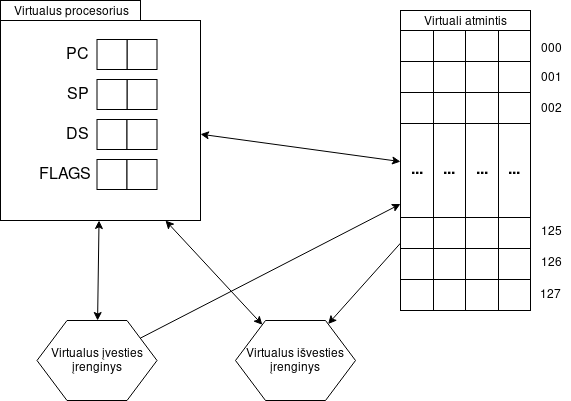
\includegraphics[width=\textwidth]{VM_model}
        \subsection{Procesorius}
            \subsubsection{Registrai}
                \paragraph{\makebox[4em][l]{PC}} Programų skaitiklis.
                \paragraph{\makebox[4em][l]{SP}} Steko nuoroda.
                \paragraph{\makebox[4em][l]{DS}} Duomenų segmento nuoroda.
                    \par
                    1 baito dydžio registras, saugantis virtualios mašinos atminties bloko numerį, kuriame prasideda duomenų segmentas.
                \paragraph{\makebox[4em][l]{FLAGS}} Paskutinės aritmetinės ar loginės operacijos požymiai. \mbox{} \\
                    \par
                    \begin{bytefield}[bitwidth=1.5em,endianness=big]{16}
                        \bitheader{0-15} \\
                        \bitbox{7}{\color{lightgray}\rule{\width}{\height}} & \bitbox{1}{CF}
                        \bitbox{3}{\color{lightgray}\rule{\width}{\height}} & \bitbox{1}{PF}
                        \bitbox{3}{\color{lightgray}\rule{\width}{\height}} & \bitbox{1}{ZF}
                    \end{bytefield}
            \subsubsection{Instrukcijų rinkinys}
                Kur nurodyta, steko argumentai išvardinti tvarka, kuria yra skaitomi iš steko.
                \paragraph{Bendros paskirties operacijos}
                    \instr{NOP}{00h}{Neatlieka jokio veiksmo.}
                    \instr{HALT}{01h}{Sustabdo procesoriaus darbą (nutraukia programos vykdymą).}
                \paragraph{Steko operacijos}
                    \instr{DUP}{10h}{Padaro steko viršūnės kopiją.}
                    \instr{POP}{11h}{Perkelia steko rodyklę po steko viršūne.}
                    \instr{POPM}{12h}{Nukopijuoja steko žodį į virtualios mašinos atmintį.}
                    \emph{Steko argumentai:} žodžio numeris virtualios mašinos atmintyje, bloko numeris virtualios mašinos atmintyje, kopijuojamas žodis.
                    \instr{PUSH imm16}{13h}{Nukopijuoja operando žodį į steką.}
                    \instr{PUSHM}{14h}{Į steką iš atminties nukopijuoja žodį.}
                    \emph{Steko argumentai:} žodžio numeris virtualios mašinos atmintyje, bloko numeris virtualios mašinos atmintyje.
                    \instr{PUSHF}{15h}{Nukopijuoja FLAGS registro reikšmę į steką.}
                    \instr{PUSHDS}{16h}{Nukopijuoja DS registro reikšmę į steką.} Naudojama, kai reikia pasiekti lokalius kintamuosius, saugomus virtualios mašinos duomenų segmente.
                \paragraph{Aritmetinės operacijos}
                    \instr{ADD}{20h}{Sudeda du steke esančius žodžius ir patalpina rezultatą steko viršūnėje.}
                    \instr{CMP}{21h}{Palygina du steke esančius žodžius.}
                    \instr{DEC}{22h}{Steko viršūnėje esančio žodžio reikšmę sumažina vienetu.}
                    \instr{DIV}{23h}{Padalina pirmąjį steke esantį žodį iš antrojo ir patalpina rezultatą steko viršūnėje.}
                    \instr{INC}{24h}{Steko viršūnėje esančio žodžio reikšmę padidina vienetu.}
                    \instr{MUL}{25h}{Sudaugina du steke esančius žodžius ir patalpina rezultatą steko viršūnėje.}
                    \instr{SUB}{26h}{Atima antrąjį steke esantį žodį iš pirmojo ir patalpina rezultatą steko viršūnėje.}
                \paragraph{Loginės operacijos}
                    \instr{AND}{30h}{Atlieka dviejų steke esančių žodžių konjunkciją ir patalpina rezultatą steko viršūnėje.}
                    \instr{NOT}{31h}{Atlieka steko viršūnėje esančio žodžio inversiją.}
                    \instr{OR}{32h}{Atlieka dviejų steke esančių žodžių disjunkciją ir patalpina rezultatą steko viršūnėje.}
                    \instr{XOR}{33h}{Atlieka dviejų steke esančių žodžių griežtą disjunkciją ir patalpina rezultatą steko viršūnėje.}
                \paragraph{Valdymo operacijos}
                    \instr{JMP}{40h}{Besąlygiškai atlieka šuolį į adresą.}
                    \emph{Steko argumentai:} \texttt{PC}-reliatyvus adresas.
                    \instr{JC}{41h}{Atlieka šuolį į adresą, kai \texttt{CF = 1}.}
                    \emph{Steko argumentai:} \texttt{PC}-reliatyvus adresas.
                    \instr{JE}{42h}{Atlieka šuolį į adresą, kai \texttt{ZF = 1}.}
                    \emph{Steko argumentai:} \texttt{PC}-reliatyvus adresas.
                    \instr{JG}{43h}{Atlieka šuolį į adresą, kai \texttt{ZF = 0} ir \texttt{CF = 1}.}
                    \emph{Steko argumentai:} \texttt{PC}-reliatyvus adresas.
                    \instr{JGE}{44h}{Atlieka šuolį į adresą, kai \texttt{ZF = 0} ir \texttt{CF = 1} arba \texttt{ZF = 1}.}
                    \emph{Steko argumentai:} \texttt{PC}-reliatyvus adresas.
                    \instr{JL}{45h}{Atlieka šuolį į adresą, kai \texttt{ZF = 0} ir \texttt{CF = 0}.}
                    \emph{Steko argumentai:} \texttt{PC}-reliatyvus adresas.
                    \instr{JLE}{46h}{Atlieka šuolį į adresą, kai \texttt{ZF = 0} ir \texttt{CF = 0} arba \texttt{ZF = 1}.}
                    \emph{Steko argumentai:} \texttt{PC}-reliatyvus adresas.
                    \instr{JNC}{47h}{Atlieka šuolį į adresą, kai \texttt{CF = 0}.}
                    \emph{Steko argumentai:} \texttt{PC}-reliatyvus adresas.
                    \instr{JNE}{48h}{Atlieka šuolį į adresą, kai \texttt{ZF = 0}.}
                    \emph{Steko argumentai:} \texttt{PC}-reliatyvus adresas.
                    \instr{JNP}{49h}{Atlieka šuolį į adresą, kai \texttt{PF = 0}.}
                    \emph{Steko argumentai:} \texttt{PC}-reliatyvus adresas.
                    \instr{JP}{4Ah}{Atlieka šuolį į adresą, kai \texttt{PF = 1}.}
                    \emph{Steko argumentai:} \texttt{PC}-reliatyvus adresas.
                    \instr{LOOP}{4Bh}{Atlieka šuolį į adresą, jei skaitiklio reikšmė didesnė už nulį.}
                    \emph{Steko argumentai:} \texttt{PC}-reliatyvus adresas, skaitiklis.
                \paragraph{Įvesties/išvesties operacijos}
                    \instr{IN}{50h}{Iš įvesties srauto į virtualios mašinos atmintį nukopijuoja ASCII koduote užkoduotus duomenis.}
                    \emph{Steko argumentai:} žodžių skaičius, žodžio numeris virtualios mašinos atmintyje, bloko numeris virtualios mašinos atmintyje.
                    \instr{INI}{51h}{Iš įvesties srauto į virtualios mašinos atmintį nukopijuoja ASCII koduote užkoduotų duomenų skaitines reikšmes.}
                    \emph{Steko argumentai:} žodžių skaičius, žodžio numeris virtualios mašinos atmintyje, bloko numeris virtualios mašinos atmintyje.
                    \instr{OUT}{52h}{Į išvesties srautą nusiunčia ASCII koduote užkoduotus duomenis.}
                    \emph{Steko argumentai:} žodžių skaičius, žodžio numeris virtualios mašinos atmintyje, bloko numeris virtualios mašinos atmintyje.
                    \instr{OUTI}{53h}{Į išvesties srautą skaitiniu pavidalu nusiunčia žodį iš steko viršūnės.}
                    \emph{Steko argumentai:} žodžių skaičius, žodžio numeris virtualios mašinos atmintyje, bloko numeris virtualios mašinos atmintyje.
                \paragraph{Darbo su bendra atminties sritimi operacijos}
                    \instr{SHREAD}{60h}{Iš bendros atminties srities nukopijuoja duomenis į virtualios mašinos atmintį.}
                    \emph{Steko argumentai:} žodžių skaičius, žodžio numeris virtualios mašinos atmintyje, bloko numeris virtualios mašinos atmintyje, žodžio numeris bendroje atminties srityje, bloko numeris bendroje atminties srityje.
                    \instr{SHWRITE}{61h}{Iš virtualios mašinos nukopijuoja duomenis į bendrą atminties sritį.}
                    \emph{Steko argumentai:} žodžių skaičius, žodžio numeris virtualios mašinos atmintyje, bloko numeris virtualios mašinos atmintyje, žodžio numeris bendroje atminties srityje, bloko numeris bendroje atminties srityje.
                \paragraph{Aparatūrinės įrangos valdymo operacijos}
                    \instr{LED}{70h}{Nustato lemputės spalvą}
                    \emph{Steko argumentai:} RGB vertės. $(0, 0, 0)$ lemputę išjungia.
        \subsection{Atmintis}
            Virtualios mašinos atmintį sudaro šešiolika vartotojo atminties blokų, kurie yra suskirstyti į segmentus pačios programos. Naudojami segmentai:
            \begin{itemize}
                \item kodo,
                \item duomenų,
                \item steko.
            \end{itemize}
            \subsubsection{Puslapiavimo mechanizmas}
                Puslapiavimo mechanizmas įgyvendinamas remiantis dviem dalykais: realios mašinos procesoriaus registru \texttt{PTR} bei virtualių mašinų puslapių lentelėmis.
        \subsection{Užduoties pavyzdys}
            Pseudokodas:
            \begin{lstlisting}[language = c]
for (i = 1; i < 3; i++) {
    if (i == 1)
        print /*“VIENAS”*/;

    if (i == 2)
        print /*“DU”*/;

    if (i == 3)
        print /*“TRYS”*/;
}
            \end{lstlisting}
            Užduoties tekstas:
            \lstset{belowskip = 0.0mm, numbers = none}
            \begin{lstlisting}
/*\$PROGRAM*/
PROGRAM NAME
/*\$DATA*/
VIENAS
DU
TRYS
/*\$CODE*/
            \end{lstlisting}
            \lstset{aboveskip = 0.0mm, belowskip = 0.0mm, numbers = left}
            \begin{lstlisting}[firstnumber = 0]
PUSH 00 01h
            \end{lstlisting}
            \begin{lstlisting}[firstnumber = 3]
DUP
PUSH 00 01h
            \end{lstlisting}
            \begin{lstlisting}[firstnumber = 7]
CMP
PUSH 00 07h
            \end{lstlisting}
            \begin{lstlisting}[firstnumber = 11]
JNE
PUSHDS
PUSH 00 00h
            \end{lstlisting}
            \begin{lstlisting}[firstnumber = 16]
PUSH 00 03h
            \end{lstlisting}
            \begin{lstlisting}[firstnumber = 19]
OUT
DUP
PUSH 00 02h
            \end{lstlisting}
            \begin{lstlisting}[firstnumber = 24]
CMP
PUSH 00 07h
            \end{lstlisting}
            \begin{lstlisting}[firstnumber = 28]
JNE
PUSHDS
PUSH 00 03h
            \end{lstlisting}
            \begin{lstlisting}[firstnumber = 33]
PUSH 00 01h
            \end{lstlisting}
            \begin{lstlisting}[firstnumber = 36]
OUT
DUP
PUSH 00 03h
            \end{lstlisting}
            \begin{lstlisting}[firstnumber = 41]
CMP
PUSH FF E0h
            \end{lstlisting}
            \begin{lstlisting}[firstnumber = 45]
JNE
PUSHDS
PUSH 00 04h
            \end{lstlisting}
            \begin{lstlisting}[firstnumber = 50]
PUSH 00 02h
            \end{lstlisting}
            \begin{lstlisting}[firstnumber = 53]
OUT
POP
HALT
        \end{lstlisting}
        \lstset{belowskip = 0.0mm, numbers = none}
        \begin{lstlisting}
/*\$END*/
        \end{lstlisting}
    \end{document}
